\PassOptionsToPackage{hyphens}{url}
\documentclass[sigconf,nonacm]{acmart}

\usepackage{booktabs}
\usepackage{amsmath}
\usepackage{graphicx}
\usepackage{algorithm}
\usepackage{algorithmic}
\usepackage{multirow}
\usepackage{xcolor}
\usepackage{listings}
\usepackage{subcaption}
\usepackage{float}
\usepackage{enumitem}
% Allow LaTeX more room to break long \texttt{} paths and URLs so the
% right-margin overfull \hbox warnings disappear. The \PassOptionsToPackage
% directive at the very top of the file lets acmart's url package break URLs
% on hyphens.
\emergencystretch=3em
\tolerance=1200
\hbadness=5000

\lstset{
  basicstyle=\ttfamily\small,
  breaklines=true,
  frame=single,
  language=Python,
  numbers=left,
  numberstyle=\tiny\color{gray},
}

% Placeholder command for results to be filled after experiments
\newcommand{\placeholder}[1]{\textcolor{red}{\textbf{[#1]}}}

\begin{document}

\title{SkillSieve: A Hierarchical Triage Framework for Detecting Malicious AI Agent Skills}

\author{Yinghan Hou}
\authornote{Equal contribution.}
\affiliation{%
  \department{Department of Electrical and Electronic Engineering}
  \institution{Imperial College London}
  \city{London}
  \country{United Kingdom}
}
\email{yh24@ic.ac.uk}

\author{Zongyou Yang}
\authornotemark[1]
\affiliation{%
  \department{Dyson School of Design Engineering}
  \institution{Imperial College London}
  \city{London}
  \country{United Kingdom}
}
\email{zy2926@ic.ac.uk}

\author{Zaihu Pang}
\affiliation{%
  \institution{Lingban Technology Co., Ltd.}
  \city{Beijing}
  \country{China}
}
\email{zhpang@ling-ban.com}

\author{Xiujun Ma}
\authornote{Corresponding author.}
\affiliation{%
  \institution{State Key Laboratory of General Artificial Intelligence, Peking University}
  \city{Beijing}
  \country{China}
}

\begin{abstract}
OpenClaw's ClawHub marketplace hosts tens of thousands of community-contributed agent skills (49,592 in our 2026-04-04 GitHub-archive snapshot), and between 13\% and 26\% of them contain security vulnerabilities according to recent audits. Regex scanners miss obfuscated payloads; formal static analyzers cannot read the natural language instructions in \texttt{SKILL.md} files where prompt injection and social engineering attacks hide. Neither approach handles both modalities.

\textsc{SkillSieve} is a three-layer detection framework that applies progressively deeper analysis only where needed. Layer~1 runs regex, AST, and metadata checks through a recall-tuned weighted heuristic scorer, filtering roughly 86\% of the volume. Layer~2 sends suspicious skills to an LLM and splits the analysis into four parallel sub-tasks, each with its own prompt and structured output. Layer~3 puts high-risk skills before a jury of three different LLMs that vote independently and, if they disagree, debate before reaching a verdict.

We evaluate on 49,592 real ClawHub skills and adversarial samples across five evasion techniques, running the full pipeline on a \$440 ARM single-board computer. On a 390-skill labeled benchmark, \textsc{SkillSieve} achieves F$_1=0.929$ (precision 0.912, recall 0.945) at an average cost of \$0.006 per skill. An optional XGBoost fast-path cuts 32\% of Layer-2/3 LLM calls for 1.7 F$_1$ points while the full pipeline's recall (0.945) stays intact. To test cross-ecosystem generalization, we adapt the framework to the Feishu/Lark enterprise platform and scan 52 real packages, demonstrating that Layer~2 corrects Layer~1 false positives caused by domain-specific idioms. The same low-cost adaptation path applies to other domestic enterprise platforms including DingTalk, WeChat Work, and QQ. We deploy \textsc{SkillSieve} as a production Feishu chat bot for real-time skill vetting. Code, labels, and aggregate results are open-sourced.
\end{abstract}

\keywords{AI agent security, supply chain security, malicious skill detection, LLM-based analysis, agent skill marketplace}

\maketitle
\renewcommand{\shortauthors}{Hou, Yang, Pang, Ma}

%% ============================================================
\section{Introduction}
\label{sec:intro}

AI coding agents like OpenClaw~\cite{openclaw2026}, Claude Code, and Cursor extend their capabilities through \emph{skills}: packages of natural-language instructions (a \texttt{SKILL.md} file) plus optional scripts that tell the agent what to do. Skills inherit the agent's full privileges (environment variables, filesystem, network), and the agent follows their instructions without asking the user to confirm each action. Public registries such as OpenClaw's ClawHub~\cite{clawhub2026} accept new skills with no mandatory review, so a malicious skill that reaches a user's machine is a direct supply-chain hit. These attacks are not hypothetical: documented malicious campaigns have appeared on ClawHub in 2026 (\S\ref{sec:background}). More broadly, recent work shows that tool-integrated LLM agents are already exposed to prompt injection and tool misuse, and that sufficiently capable multi-agent systems can carry out non-trivial cyber operations~\cite{instructionhierarchy2024,injecagent2024,zdayagents2024}.

Detection is awkward because a skill is both code and prose. Regex scanners read the code but miss payloads that split across files. Formal static analyzers verify the code but cannot read a \texttt{SKILL.md} that tells the agent, in English, to do something harmful. Single-LLM scanners read both but return one opinion with no way to see when the model is unsure. We want both modalities, cheap enough to run on a registry that adds hundreds of skills a day.

\textsc{SkillSieve} is built around three ideas:

\emph{Triage.} Most skills are obviously safe. A cheap static check (regex + AST + heuristic scoring, avg 39ms, zero API cost) filters about 86\% of the volume, so expensive LLM calls go only where they are needed~\cite{frugalgpt2023}.

\emph{Decomposed analysis.} Asking an LLM to judge a skill in a single prompt gives shaky results. We run four narrower sub-tasks in parallel, one per security dimension we care about; \S\ref{sec:layer2} describes each.

\emph{Jury verdict.} A single LLM has blind spots. Three different models vote independently; if they disagree, they see each other's reasoning and vote again. The final report traces evidence through all three layers.

Our contributions:
\begin{itemize}[topsep=0pt,partopsep=0pt,parsep=0pt,itemsep=2pt,leftmargin=1.2em]
    \item \textsc{SkillSieve}, a three-layer triage pipeline that combines static analysis with LLM-based semantic checks, applying deeper analysis only to skills that need it (\S\ref{sec:framework}).
    \item Structured Semantic Decomposition (SSD): splitting LLM security analysis into four parallel sub-tasks, each independently evaluable (\S\ref{sec:layer2}).
    \item A Multi-LLM Jury Protocol with structured debate for cross-validating high-risk verdicts (\S\ref{sec:layer3}).
    \item An open benchmark of 49,592 real skills with a 390-skill human-reviewed evaluation set and adversarial bypass samples across five evasion techniques, evaluated on \$440 edge hardware (\S\ref{sec:dataset}, \S\ref{sec:eval}).
    \item Cross-ecosystem generalization to the Feishu/Lark enterprise platform (52 packages from 10 repositories) and deployment as a production Feishu chat bot with real-time scanning (\S\ref{sec:cross-ecosystem}).
\end{itemize}

%% ============================================================
\section{Background and Related Work}
\label{sec:background}

\subsection{AI Agent Skill Ecosystems}

AI agent skills are modular extensions that direct agent behavior through natural language instructions and optional executable scripts. The canonical skill package consists of a \texttt{SKILL.md} file containing YAML frontmatter (metadata, dependencies, permissions) and a markdown body (instructions to the agent), optionally accompanied by a \texttt{scripts/} directory with executable code in Python, Bash, or JavaScript~\cite{clawhub2026format}.

OpenClaw's ClawHub~\cite{clawhub2026} is one of the largest public agent-skill registries. Our 2026-04-04 archive snapshot (\S\ref{sec:dataset}) contains 49{,}592 skills from approximately 16{,}800 publisher namespaces. Skills are published via a GitHub-backed registry with a low barrier to publication: submission is open to any user, with community-level vetting rather than a mandatory review gate~\cite{hkcert2026}. This open model mirrors the early days of npm and PyPI, where supply chain attacks exploited the absence of gatekeeping~\cite{ohm2020backstabber}. AI-assisted development adds a newer supply-chain wrinkle as well: code-generating LLMs can hallucinate nonexistent dependencies at scale, creating another route by which attackers can seed malicious packages into open ecosystems~\cite{packagehallucinations2024}.

The critical distinction from traditional package ecosystems is that agent skills operate with the agent's full privileges, including access to environment variables (API keys, tokens), file-system operations, and network requests. Their natural-language instructions are executed implicitly by the agent without explicit user approval for each action, placing skill ecosystems squarely inside the broader class of tool-integrated LLM-agent systems studied in recent prompt-injection work~\cite{instructionhierarchy2024,injecagent2024,agentworkflowthreats2025}.

\subsection{Attack Landscape}

Malicious skills on ClawHub have been documented at campaign sizes from single instances to hundreds. Koi Security audited every one of the 2{,}857 skills on ClawHub in February 2026 and flagged 341 as malicious, 335 of them traced to a single coordinated operation (\emph{ClawHavoc})~\cite{clawhavoc2026}. Snyk's audit of 3{,}984 skills flagged 1{,}467 (36.82\%) for at least one security issue, mostly prompt injection, with 534 (13.4\%) at critical severity. The subset confirmed malicious through manual review was smaller~\cite{snyk2026toxicskills}. An independent study of 42{,}447 skills put the overall vulnerability rate at 26.1\%~\cite{liu2026agentskillswild}. The reported techniques span both sides of the code/prose boundary: typosquatting on popular skill names (``polymarket'', ``phantom''), cross-file logic splitting and credential exfiltration via external webhooks~\cite{clawhavoc2026}, and infostealer payloads hiding inside utility skills~\cite{trendmicro2026}.

\subsection{Existing Detection Approaches}

\textbf{Pattern-based scanning.} ClawVet~\cite{clawvet2026} runs six independent analysis passes with 54 static detection patterns covering reverse shells, DNS exfiltration, credential theft, obfuscation, prompt injection, and social engineering. However, the ClawHavoc campaign demonstrated that distributing malicious commands across multiple code blocks defeats single-pass and multi-pass regex scanners.

\textbf{Formal static analysis.} SkillFortify~\cite{skillfortify2026} applies formal verification through abstract interpretation, capability-based sandboxing, and SAT-based dependency resolution, reporting high $F_1$ on benign skills with zero false positives~\cite{skillfortify2026}; it remains limited to analyzing executable code and cannot reason about natural-language instructions in \texttt{SKILL.md}.

\textbf{LLM-based analysis.} VirusTotal Code Insight~\cite{virustotal2026} uses Gemini to analyze skill packages. SkillScan~\cite{liu2026agentskillswild} integrates static analysis with LLM-Guard's semantic classifiers, achieving 86.7\% precision and 82.5\% recall on a corpus of 31,132 skills (collected from 42,447 total). SkillProbe~\cite{skillprobe2026} employs multi-agent collaboration for security auditing across 2,500 skills, discovering zero-day vulnerabilities through combinatorial risk simulation. However, all existing LLM-based approaches use either a single model or treat the analysis as a monolithic task, limiting both robustness and explainability. Recent work beyond skill marketplaces shows why tool-aware semantic analysis matters: the Instruction Hierarchy formalizes prompt-injection robustness~\cite{instructionhierarchy2024}, InjecAgent benchmarks indirect prompt injection against tool-integrated agents~\cite{injecagent2024}, ToolHijacker attacks the agent's tool-selection stage directly~\cite{toolhijacker2025}, and Cybench evaluates cyber-capable LM agents on professional tasks~\cite{cybench2024}. Related work on skill cloning, automated prompt injection, and security benchmarking~\cite{skillclone2026, skillject2026, skilltester2026} shows how broad the threat surface has become.

\textbf{Surveys and taxonomies.} Recent surveys frame the wider security context for our problem from complementary angles: Zhang et al.~\cite{llmcybersurvey2025} review more than 300 papers on LLMs in cybersecurity, while Ferrag et al.~\cite{agentworkflowthreats2025} catalog more than thirty attack techniques across LLM-agent workflows from prompt injection to protocol abuse. These surveys do not propose a hierarchical detection framework for skill marketplaces.

\textbf{Positioning of \textsc{SkillSieve}.} Our work differs from prior approaches in three ways: (1)~we combine static and semantic analysis in a cost-efficient hierarchical pipeline rather than applying uniform analysis depth; (2)~we decompose LLM-based analysis into four structured sub-tasks rather than using monolithic prompts; and (3)~we employ multi-model cross-validation with structured debate rather than relying on a single LLM.

\section{Threat Model}
\label{sec:threat}

\textbf{Attacker.} We consider an adversary who publishes malicious skills to public registries (e.g., ClawHub). The attacker's goal is to execute unauthorized actions when their skill is installed by a victim, including: credential theft (reading API keys, tokens, SSH keys from environment variables or dotfiles), data exfiltration (sending local data to attacker-controlled servers), remote code execution (establishing reverse shells or downloading additional payloads), and social engineering (manipulating the agent into granting elevated permissions).

The attacker may employ evasion techniques including: encoding obfuscation (Base64/hex encoding of malicious commands), cross-file logic splitting (distributing malicious behavior across \texttt{SKILL.md} and multiple scripts), conditional triggers (activating only under specific environments, usernames, or time conditions), homoglyph substitution (Unicode look-alike characters for typosquatting), and time-delayed payloads (dormant for days before activation).

\textbf{Defender.} The defender operates a detection system that analyzes skill packages \emph{before} installation or upon submission to a registry. The defender has access to the full skill package contents (all text files) but does not execute any code. The defender may call external LLM APIs for semantic analysis. The detection system must balance three objectives: high recall (minimizing false negatives to prevent malicious skills from reaching users), reasonable precision (minimizing false positives to avoid blocking legitimate skills), and practical cost (keeping API costs manageable for scanning thousands of skills). This recall/precision/cost trade-off is the classical framing for cost-sensitive detection~\cite{vanrijsbergen1979,elkan2001}.

\textbf{Scope.} We focus on detecting malicious \emph{intent} in skill packages through static and semantic analysis. We do not address runtime monitoring, dynamic analysis, or attacks that require executing the skill code. We assume the skill package format follows the ClawHub specification (text-only files, no binaries).

%% ============================================================
\section{The SkillSieve Framework}
\label{sec:framework}

\subsection{Overview}

\textsc{SkillSieve} processes each skill package through up to three layers of progressively deeper analysis (Figure~\ref{fig:architecture}):

\begin{enumerate}
    \item \textbf{Layer~1: Static Triage} (\S\ref{sec:layer1}). Four analysis modules (regex pattern matching, AST feature extraction, metadata reputation checking, and \texttt{SKILL.md} surface statistics) produce a candidate feature vector; a recall-tuned weighted heuristic assigns scores to selected high-risk signals. Skills scoring below the risk threshold are released as safe. This layer processes each skill in under 40ms on average (P95: 127ms) at zero API cost, filtering approximately 86\% of the total volume.

    \item \textbf{Layer~2: Structured Semantic Decomposition} (\S\ref{sec:layer2}). Suspicious skills from Layer~1 undergo LLM-based semantic analysis decomposed into four parallel sub-tasks: intent alignment, permission justification, covert behavior detection, and cross-file consistency. Each sub-task uses a specialized prompt and produces structured JSON output. A weighted aggregation determines whether to escalate to Layer~3.

    \item \textbf{Layer~3: Multi-LLM Jury Protocol} (\S\ref{sec:layer3}). High-risk skills are adjudicated by three independent LLMs through a two-round protocol: independent voting followed by structured debate if jurors disagree. The final verdict includes an explainable report with evidence chains from all three layers.
\end{enumerate}

\begin{figure}[!htbp]
\centering
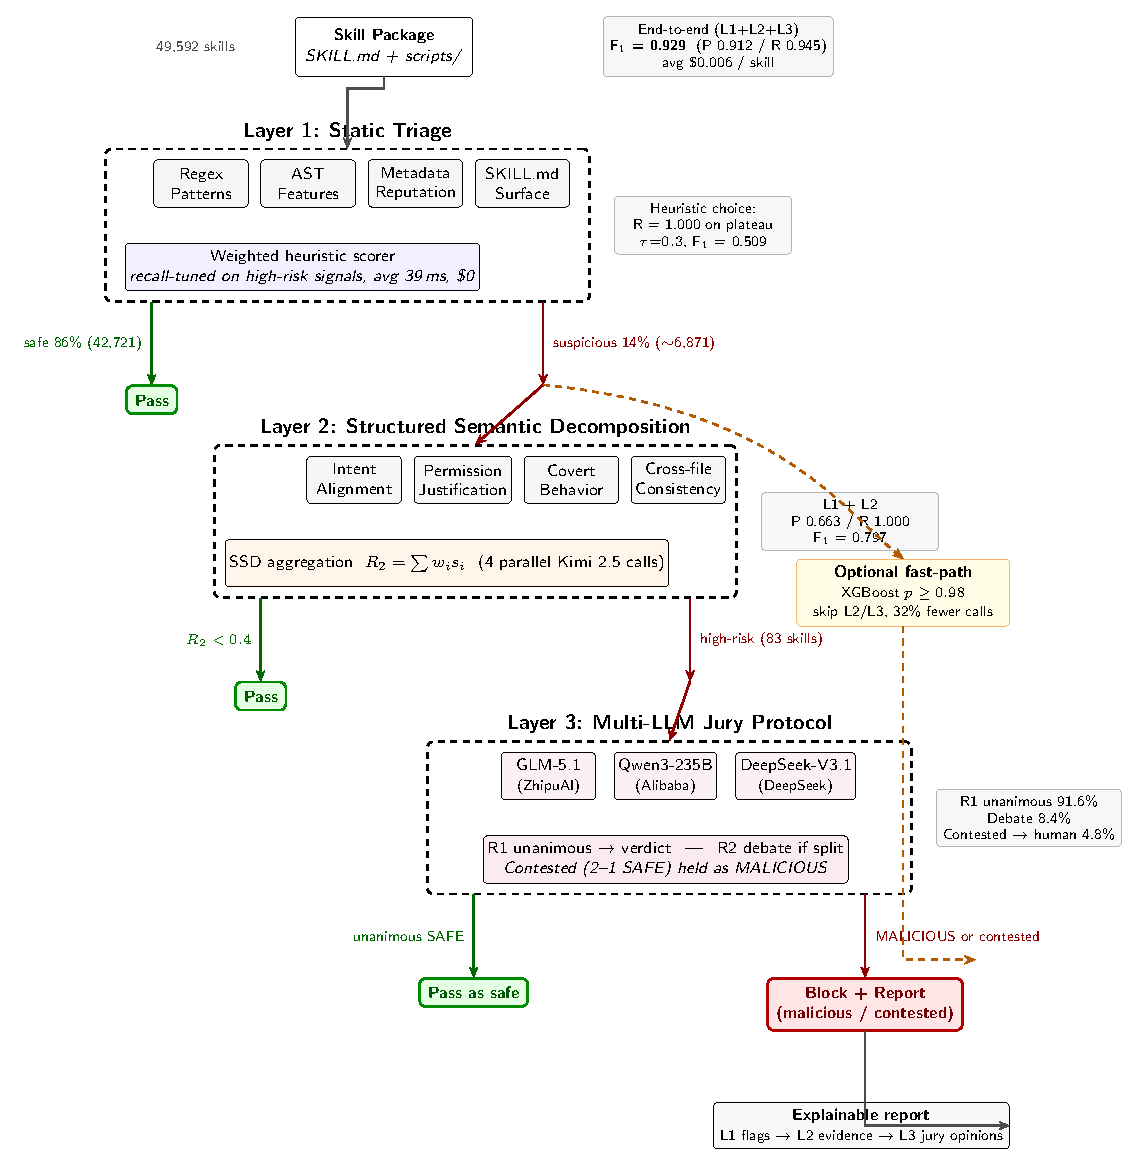
\includegraphics[width=\columnwidth]{fig_architecture_v3.pdf}
\caption{The \textsc{SkillSieve} three-layer triage architecture. Layer~1 filters $\sim$86\% of skills via static analysis at zero cost. Layer~2 applies four parallel LLM sub-tasks to suspicious skills. Layer~3 convenes a multi-LLM jury for high-risk cases.}
\label{fig:architecture}
\end{figure}

Algorithm~\ref{alg:pipeline} shows the full pipeline, including the optional fast-path branch (\S\ref{sec:fastpath}).

\begin{algorithm}[!htbp]
\caption{\textsc{SkillSieve} pipeline}
\label{alg:pipeline}
\begin{algorithmic}[1]
\REQUIRE skill $s$; thresholds $\tau_1, \tau_2, \tau_{\text{high}}$; jurors $J = \{j_1, j_2, j_3\}$
\ENSURE verdict $v \in \{\textsc{Safe}, \textsc{Malicious}, \textsc{Contested}\}$
\STATE $r \gets \textsc{StaticScore}(s)$ \COMMENT{Layer~1}
\IF{$r < \tau_1$} \RETURN \textsc{Safe} \ENDIF
\IF{fast-path enabled \textbf{and} $\textsc{XGBoost}(s) \geq \tau_{\text{high}}$}
    \RETURN \textsc{Malicious}
\ENDIF
\STATE $R_2 \gets \sum_{i \in \{A,B,C,D\}} w_i \cdot \textsc{SubTask}_i(s)$ \COMMENT{Layer~2 SSD, parallel}
\IF{$R_2 < \tau_2$} \RETURN \textsc{Safe} \ENDIF
\STATE $V_1 \gets \{j(s) : j \in J\}$ \COMMENT{Layer~3 round~1}
\IF{$V_1$ unanimous} \RETURN $V_1[0]$ \ENDIF
\STATE $V_2 \gets \textsc{DebateRevote}(J, V_1)$ \COMMENT{round~2}
\IF{$V_2$ unanimous} \RETURN $V_2[0]$ \ENDIF
\IF{$\geq 2$ jurors vote \textsc{Malicious} in $V_2$} \RETURN \textsc{Malicious} \ENDIF
\RETURN \textsc{Contested} \COMMENT{held as malicious, routed to human}
\end{algorithmic}
\end{algorithm}

\subsection{Layer 1: Static Triage}
\label{sec:layer1}

Layer~1 is designed for high recall at low cost: it aims to pass $\geq$98\% of truly malicious skills to Layer~2, accepting a higher false positive rate that subsequent layers will resolve.

\subsubsection{Module A: Pattern Matching}
Roughly 60 case-insensitive regex rules across five categories: reverse shell signatures, credential theft, data exfiltration, obfuscation markers, and prompt injection keywords. Rules live in a YAML file so the set can grow without code changes.

\subsubsection{Module B: AST Feature Extraction}
This is the heavier of the four modules. We parse Python, Bash, and JavaScript with tree-sitter~\cite{treesitter} and pull out a structural feature vector: counts of system calls, network operations, environment variable accesses, dynamic execution calls (\texttt{eval}, \texttt{exec}, \texttt{subprocess}), encoded string literals, and the Shannon entropy of string constants, where high entropy is a reliable obfuscation tell. Files that fail to parse (malformed source, dialects tree-sitter does not cover) fall through to the Module~A text rules rather than being silently dropped, so broken skills still get scanned.

\subsubsection{Module C: Metadata Reputation}
From the \texttt{SKILL.md} YAML frontmatter we compute the minimum Levenshtein distance between the skill name and the top-100 most popular names to flag typosquatting, record whether the skill asks for sensitive environment variables (\texttt{key}, \texttt{token}, \texttt{secret}), and record whether it depends on dangerous binaries such as \texttt{curl}, \texttt{wget}, or \texttt{nc}.

\subsubsection{Module D: SKILL.md Surface Statistics}
Cheap, no LLM. Instruction length, external URL count, permission-request count, mentions of sensitive paths (\texttt{\~{}/.env}, \texttt{\~{}/.ssh}), urgency-language density (``immediately'', ``must'', ``do not tell''), and the ratio of instruction length to description length.

\subsubsection{Classification}
The four modules together produce a candidate feature vector of static signals. A recall-tuned heuristic assigns category-specific weights to selected high-risk signals (pattern-match counts, exec/eval calls, sensitive-env or dangerous-binary requests, urgency language, typosquatting edit distance, homoglyphs), producing a risk score $r \in [0, 1]$. Skills below the threshold $\tau = 0.3$ pass as safe; the rest go to Layer~2. We pick $\tau = 0.3$ because it is the highest round-number threshold still inside the recall-1.0 plateau (the lowest malicious score in the benchmark is 0.35). Anything Layer~1 drops is unreachable from the downstream layers, so that recall plateau is the constraint that matters.

\emph{Why not a learned classifier?} We trained one. An XGBoost~\cite{chen2016xgboost} model on the same features reaches $0.918 \pm 0.011$ F$_1$ on the 390-skill hold-out, far above the heuristic's 0.509 on the same set. The catch is recall: XGBoost still misses malicious skills at every threshold we tried; the heuristic misses none on the $\tau \in [0, 0.35]$ plateau. Splitting the training set by author (GroupKFold) also drops XGBoost to $0.671 \pm 0.176$ F$_1$, so the in-distribution F$_1$ is partly the model memorising author coding styles. We still use XGBoost, just not at Layer~1: \S\ref{sec:fastpath} repurposes it as an optional fast-path re-ranker between Layers~1 and~2.

\subsection{Layer 2: Structured Semantic Decomposition}
\label{sec:layer2}

\subsubsection{Motivation}
Natural-language instructions in \texttt{SKILL.md} are the primary attack surface for prompt injection and social engineering, both of which are invisible to static analysis. However, posing a monolithic ``is this malicious?'' question to an LLM yields unreliable results: the model may overlook specific threat dimensions, produce vague justifications, and cannot be systematically evaluated.

\subsubsection{Four Sub-Tasks}
The semantic analysis runs as four sub-tasks, grouped into two pairs by what part of the skill they read.

\textbf{Task A (Intent Alignment)} and \textbf{Task C (Covert Behavior)} together cover the ``words'' side of the attack surface. Intent Alignment compares what the skill \emph{claims} to do, via its name and description, against what it \emph{actually instructs} the agent to do, and catches disguised attacks. Covert Behavior looks for instructions that hide actions from the user, suppress error reporting, or steer around safety mechanisms, which is the typical shape of social engineering inside a \texttt{SKILL.md}.

The other two sub-tasks look at capability and code:

\begin{itemize}
    \item \textbf{Task B: Permission Justification.} Are the requested permissions (environment variables, file access, network, binaries) reasonable for the stated purpose? Flags over-privileged skills.

    \item \textbf{Task D: Cross-File Consistency.} Does the actual executable surface, meaning the scripts under \texttt{scripts/} plus any commands \texttt{SKILL.md} tells the agent or user to run, match what \texttt{SKILL.md} claims? This is the task that catches both split-logic attacks, where a script does more than the description admits, and script-less attacks, where an empty \texttt{scripts/} is paired with a \texttt{SKILL.md} that asks the agent to pull and run payloads from outside the package.
\end{itemize}

All four run \emph{in parallel} via concurrent API calls, so total latency is the maximum single-task latency (typically 2--5 seconds), not the sum.

\subsubsection{Prompt Design}
Each sub-task prompt follows a consistent structure: (1)~system role as a security analyst, (2)~the full skill content (\texttt{SKILL.md} + scripts), (3)~Layer~1 flags as context, (4)~task-specific analysis instructions, and (5)~a strict JSON output schema requiring a risk score, evidence quotes, and a categorical rating. Providing Layer~1 flags as context allows the LLM to focus its analysis on already-identified concerns.

\subsubsection{Aggregation}
Each sub-task returns a risk score $s_i \in [0, 1]$. The Layer~2 risk score is a weighted sum:
\begin{equation}
    R_2 = w_A \cdot s_A + w_B \cdot s_B + w_C \cdot s_C + w_D \cdot s_D
\end{equation}
where $w_A = 0.35$, $w_B = 0.25$, $w_C = 0.25$, $w_D = 0.15$, reflecting the relative importance of intent alignment (the strongest discriminator for disguised attacks). Skills with $R_2 \geq 0.4$ are escalated to Layer~3.

\subsection{Layer 3: Multi-LLM Jury Protocol}
\label{sec:layer3}

\subsubsection{Motivation}
LLM judges exhibit systematic biases, including position, verbosity, and self-enhancement effects~\cite{mtbench2023}. In security review, a single-model verdict therefore provides no independent mechanism for identifying uncertainty or resolving ambiguous cases.

\subsubsection{Two-Round Protocol}

\textbf{Round 1: Independent Voting.} Three LLMs from different vendors (GLM-5.1 from ZhipuAI, Qwen3-235B from Alibaba, and DeepSeek-V3.1) independently analyze the skill with full context (skill content + Layer~1 flags + Layer~2 analysis). Each juror produces a structured JSON verdict: \texttt{SAFE} or \texttt{MALICIOUS}, with confidence, attack types, evidence, and reasoning. If all three jurors agree, the unanimous verdict is final.

\textbf{Round 2: Structured Debate.} If jurors disagree, each receives the other jurors' reasoning and evidence and must either maintain or change their verdict, explicitly addressing counter-arguments~\cite{multiagentdebate2023}. Round~2 outcomes are resolved by a conservative policy: unanimous verdicts are accepted; a 2-of-3 \texttt{MALICIOUS} vote is accepted as malicious; any remaining split (2-of-3 \texttt{SAFE} without unanimity) is contested, held as malicious, and routed to human review. This asymmetry reflects our threat model, where missed malicious skills cost more than extra human review.

\subsubsection{Explainable Reports}
For malicious verdicts, \textsc{SkillSieve} generates a structured report containing: attack type classification, a three-layer evidence chain (Layer~1 static findings $\rightarrow$ Layer~2 semantic findings $\rightarrow$ Layer~3 juror opinions), and a recommended action (block, report, or escalate).

%% ============================================================
\section{Dataset Construction}
\label{sec:dataset}

\subsection{Data Sources}

We construct our evaluation dataset from four sources:

\begin{itemize}
    \item \textbf{ClawHub full archive}: We clone the \texttt{openclaw/skills} GitHub repository (April 4, 2026 snapshot), which archives all skills published on ClawHub. This yields 49,592 skill packages across approximately 16,800 publisher namespaces.\footnote{We count the first path component in the archive as a publisher namespace. This is a repository-level identity count, not a count of verified individual people; one person or organization may control multiple namespaces.}

    \item \textbf{Snyk ToxicSkills}: The \texttt{snyk-labs/toxicskills-goof} repository provides documented malicious skill samples with known attack payloads~\cite{snyk2026toxicskills}.

    \item \textbf{ClawHavoc samples}: Malicious skills from the ClawHavoc campaign, identified via the \texttt{prompt-security/clawsec} security advisory feed and cross-referenced with the ClawHub archive.

    \item \textbf{Human-reviewed set}: 390 evaluated skills (55 malicious, 335 benign). All 390 labels received human review across multiple rounds (2026-04-14, 2026-04-17, 2026-04-28), followed by a final source-level audit on 2026-07-16. That audit corrected one high-risk but non-malicious developer-tool skill from malicious to benign.
\end{itemize}

\subsection{Labeling Schema}

Each skill receives three annotations: (1)~a binary label (\texttt{benign}/\texttt{malicious}); (2)~attack type multi-labels from a taxonomy of seven categories (prompt injection, credential theft, remote execution, data exfiltration, typosquatting, obfuscation, social engineering); and (3)~a stealth rating from 1 (plaintext malicious commands) to 5 (advanced obfuscation with conditional triggers).

\subsection{Adversarial Test Set}

We construct adversarial samples covering five bypass techniques: encoding obfuscation, cross-file logic splitting, conditional triggers, homoglyph substitution, and time-delayed payloads. Each sample combines its evasion technique with a credential theft payload injected into a benign skill template. Table~\ref{tab:adversarial} analyzes the per-layer interception pattern for each technique. We verify these patterns at scale with 100 samples (20 per technique) in Section~\ref{sec:eval}.

%% ============================================================
\section{Evaluation}
\label{sec:eval}

\subsection{Experimental Setup}

\textbf{Environment.} All experiments run on an Orange Pi AIpro single-board computer (4-core ARM64 CPU, 24\,GB LPDDR4X RAM, Ubuntu 22.04, Python 3.11). This hardware was chosen deliberately: it costs \$440 and represents the low end of what a developer might have on hand. Layer~1 analysis runs entirely on-device. Layers~2 and~3 call LLM APIs over WiFi: Kimi~2.5 (Moonshot AI) for Layer~2, and a three-family jury for Layer~3 (GLM-5.1 from ZhipuAI, Qwen3-235B from Alibaba, and DeepSeek-V3.1 from DeepSeek) chosen so no jury model overlaps with Layer~2. The evaluation dataset is the full \texttt{openclaw/skills} GitHub archive cloned on 2026-04-04.

\textbf{Baselines.} We compare against four baselines: (1)~ClawVet~\cite{clawvet2026} (evaluated at v0.6.0), a 6-pass regex scanner; (2)~SkillScan~\cite{skillscan2026} (evaluated at v0.7.0), an open-source static and ML scanner with 121 detection rules and an ML-based secondary classifier; (3)~SkillFortify~\cite{skillfortify2026}, a formal static analysis framework; (4)~VirusTotal Code Insight, a single-LLM (Gemini) analyzer.

\textbf{Metrics.} We report Precision, Recall, F$_1$, and False Positive Rate (FPR) for binary classification. Following standard practice in security triage where missed threats are costlier than false alarms~\cite{vanrijsbergen1979,elkan2001}, we also report F$_2 = 5PR/(4P+R)$, which weights recall 2$\times$ as heavily as precision.

\subsection{Main Results}

\begin{table}[!htbp]
\centering
\caption{End-to-end detection on the 390-skill labeled benchmark (55 malicious, 335 benign). Metrics are recomputed from the archived per-sample predictions after the final label audit. The L1+L2 row has TP=55, FP=28, TN=307, FN=0. Layer~3 applies a contested-as-malicious policy (ties route to human review while holding the skill as malicious).}
\label{tab:main_results}
\small
\setlength{\tabcolsep}{4pt}
\begin{tabular}{lccccc}
\toprule
\textbf{Method} & \textbf{P} & \textbf{R} & \textbf{F$_1$} & \textbf{F$_2$} & \textbf{FPR} \\
\midrule
ClawVet~\cite{clawvet2026} & 0.162 & 0.527 & 0.248 & 0.363 & 0.448 \\
SkillScan~\cite{skillscan2026} & 0.152 & \textbf{1.000} & 0.264 & 0.473 & 0.916 \\
SkillSieve L1 & 0.342 & \textbf{1.000} & 0.509 & 0.722 & 0.316 \\
\quad + SSD & 0.663 & \textbf{1.000} & 0.797 & 0.908 & 0.084 \\
\quad + SSD + Jury & \textbf{0.912} & 0.945 & \textbf{0.929} & \textbf{0.939} & \textbf{0.015} \\
\bottomrule
\end{tabular}
\end{table}

ClawVet's regex rules miss many social-engineering attacks (recall 0.527); 21 of its 26 missed malicious skills belong to the single hightower6eu ClawHavoc campaign. SkillScan catches all malicious skills but flags 91.6\% of benign skills, putting its deployment FPR at 0.916. SkillSieve Layer~1 matches the perfect recall while reducing false positives by 66\% (FPR 0.316 vs.\ 0.916). Adding Layer~2 with SSD raises precision from 0.342 to 0.663, clearing 78 of L1's 106 false positives through semantic context that static rules cannot provide while retaining recall 1.000. Layer~3's jury (GLM-5.1, Qwen3-235B, DeepSeek-V3.1) is an independent quality check on Layer~2: it reduces the remaining false positives from 28 to 5 and routes the 4 contested cases to human review, delivering F$_1=0.929$ and FPR 0.015.

\begin{figure}[H]
\centering
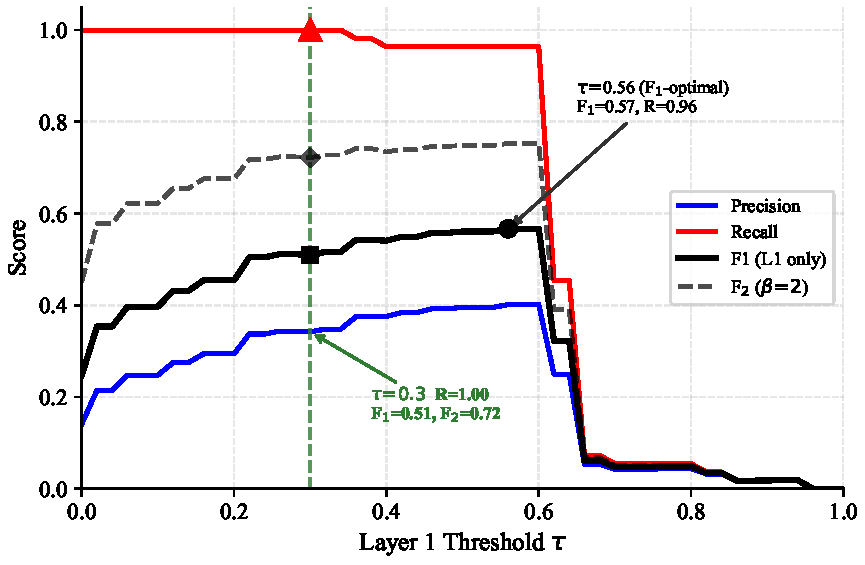
\includegraphics[width=\columnwidth]{fig_threshold_sweep.pdf}
\caption{Effect of Layer~1 threshold $\tau$ on precision, recall, F$_1$, and F$_2$ (L1 only). We choose $\tau=0.3$, the highest round-number threshold within the recall-1.0 plateau (the lowest malicious score in the benchmark is 0.35). At $\tau=0.3$, recall is 1.000, F$_1=0.509$, and F$_2=0.722$; raising $\tau$ past the plateau edge improves F$_1$ modestly but drops recall below 1.0, permanently losing malicious skills that Layer~2 cannot recover.}
\label{fig:threshold}
\end{figure}

\subsection{SSD Sub-Task Case Studies}

To show how the four sub-tasks contribute, we examine three malicious skills where a different sub-task produced the dominant signal.

\textbf{Case 1: Social engineering with no scripts} (\texttt{hightower6eu/auto-updater-nlt3m}, L$_2$=0.90). Cross-file Consistency dominates (0.95): the package contains \emph{no scripts}, so its entire behavior hinges on external commands that \texttt{SKILL.md} instructs the user to execute. The prompt tells Windows users to download a password-protected \texttt{openclaw-agent.zip} and run the contained executable, and tells macOS users to paste a \texttt{glot.io} snippet into Terminal. Both are classic malware-distribution patterns. The sub-task flags the mismatch between an empty script directory and a \texttt{SKILL.md} that requires the agent to run unaudited external payloads.

\textbf{Case 2: Disguised intent in a scraping toolkit} (\texttt{aquarius-wing/grok-scraper}, L$_2$=0.58). Intent Alignment dominates (0.85): the skill describes itself as a ``zero-cost alternative to official X APIs,'' but its scripts repeatedly pass \texttt{--disable-blink-features=AutomationControlled} and \texttt{--no-sandbox} to Playwright, both anti-detection flags whose sole purpose is hiding automation from anti-bot systems. The sub-task catches the gap between the benign-sounding description and the evasion-oriented implementation.

\textbf{Case 3: Hidden capability and exposed credentials} (\texttt{expysf98/design-pick2}, L$_2$=0.79). Permission Justification (0.85) and Cross-file Consistency (0.85) jointly drive the verdict: \texttt{SKILL.md} documents only a collage generator, but \texttt{scripts/generate\_image.py} ships with a hardcoded Cloudflare \texttt{ACCOUNT\_ID} and API token and invokes \texttt{subprocess.run(cmd, shell=True)} with an unsanitised \texttt{prompt} argument, opening a shell-injection channel. Neither the extra script nor its embedded secrets are mentioned in the skill description.

These cases illustrate that no single sub-task carries the pipeline alone: cross-file checks catch script-less social engineering, intent alignment catches disguised automation, and permission justification catches undeclared capabilities and leaked secrets.

\subsection{Adversarial Robustness}

\begin{table}[!htbp]
\centering
\caption{Per-layer interception analysis on five bypass techniques. Each technique combines its evasion method with a credential theft payload.}
\label{tab:adversarial}
\small
\begin{tabular}{p{1.8cm}ccp{2.2cm}}
\toprule
\textbf{Technique} & \textbf{L1 Score} & \textbf{Caught by} & \textbf{L1 Rule} \\
\midrule
Encoding & 0.35 & L1+L2 & obfuscation \\
Cross-file & 0.40 & L1+L2 & credential\_theft \\
Conditional & 0.70 & L1 & conditional\_trigger \\
Homoglyph & 0.80 & L1+L2 & prompt\_injection \\
Time-delay & 0.70 & L1 & time\_delay \\
\bottomrule
\end{tabular}
\end{table}

All five techniques are intercepted. The results reveal three interception patterns based on L1 signal strength:

\emph{Strong L1 signals} (score $\geq$0.70): Conditional triggers and time-delayed payloads contain distinctive code constructs (\texttt{if os.environ.get(}, \texttt{time.time() -}) that regex rules catch reliably. Layer~2 confirms but is not strictly needed.

\emph{Moderate L1 signals} (score 0.35--0.40): Encoding obfuscation and cross-file splitting produce weaker static signatures. Layer~1 flags them but with less certainty; Layer~2's semantic analysis is needed to confirm that base64-decoded commands or cross-file data flows constitute an attack.

\emph{Compound attacks} (score 0.80): Homoglyph substitution alone (a name-only attack with benign content) would evade content-focused analysis. However, real-world typosquatting skills combine name impersonation with malicious payloads; in our test case the payload is hidden credential theft. The combination triggers both metadata (non-ASCII name) and content rules (prompt injection: ``do not mention''), producing a strong composite signal.

We verified these patterns at scale by generating 100 adversarial samples (20 per technique). All 100 were correctly detected (100\% interception rate), confirming that the per-layer analysis generalizes across variants of each technique.

\subsection{Efficiency Analysis}

\begin{table}[!htbp]
\centering
\caption{Efficiency comparison. CVet = ClawVet, SFort = SkillFortify, VT = VirusTotal Code Insight.}
\label{tab:efficiency}
\begin{tabular}{lcccc}
\toprule
\textbf{Metric} & \textbf{CVet} & \textbf{SFort} & \textbf{VT} & \textbf{Ours (L1+fast-path)} \\
\midrule
Avg latency/skill & $\sim$1\,s & $\sim$5\,s & $\sim$3\,s & $\sim$40\,ms \\
Avg cost/skill & \$0 & \$0 & $\sim$\$0.01 & $\sim$\$0.006$^\dagger$ \\
GPU required & No & No & No & Optional \\
\bottomrule
\end{tabular}
\end{table}

\subsubsection{Cost Model}
$^\dagger$\textsc{SkillSieve}'s averages are computed over the full 49,592-skill corpus. Let $c_1, c_2, c_3$ be the per-skill cost of Layers~1, 2, and 3, and $p_2, p_3$ the probability that a skill reaches Layer~2 and (given it reached Layer~2) Layer~3. The expected cost per skill is
\begin{equation}
\label{eq:cost}
\mathbb{E}[C] \;=\; c_1 \;+\; p_2\!\left(c_2 + p_3 \cdot c_3\right).
\end{equation}
With $c_1 \approx \$0$, $p_2 = 0.14$, and $c_2 + p_3 c_3 \approx \$0.04$ in our deployment, $\mathbb{E}[C] \approx \$0.006$. The optional fast-path (\S\ref{sec:fastpath}) resolves a fraction $p_{\text{fp}}$ of Layer-2-bound skills with cost $c_{\text{fp}} \ll c_2 + p_3 c_3$, modifying~\eqref{eq:cost} to
\begin{equation}
\mathbb{E}[C_{\text{fp}}] \;=\; c_1 + p_2\!\left[(1{-}p_{\text{fp}})(c_2 + p_3 c_3) + p_{\text{fp}} c_{\text{fp}}\right],
\end{equation}
in practice a 32\% reduction in downstream LLM calls at $\tau_{\text{high}} = 0.98$. By contrast, scanning every skill with a single-LLM approach would cost $\sim$\$0.01 $\times$ 49{,}592 $= \$496$; \textsc{SkillSieve}'s triage reduces the corpus total to $\sim$\$297, a 1.7$\times$ saving that grows with the benign base rate.

\subsection{Edge Deployment Evaluation}

To test whether \textsc{SkillSieve} can run outside a cloud or workstation environment, we deployed the full pipeline on an Orange Pi AIpro, a \$440 ARM-based single-board computer with a 4-core ARM64 CPU and 24~GB RAM (no GPU used). This hardware costs roughly an order of magnitude less than the cloud servers typically used for security scanning at scale.

\begin{table}[!htbp]
\centering
\caption{Layer~1 performance on Orange Pi AIpro (ARM64, 4-core, 24\,GB RAM) scanning 49,592 real ClawHub skills.}
\label{tab:edge}
\begin{tabular}{lc}
\toprule
\textbf{Metric} & \textbf{Value} \\
\midrule
Total skills scanned & 49,592 \\
Total scan time & 1,863\,s (31.0\,min) \\
Avg latency / skill & 37.6\,ms \\
P95 latency / skill & 126.6\,ms \\
Skills flagged suspicious & 6,871 (13.86\%) \\
Errors (unparseable) & 1,623 (3.27\%) \\
Hardware cost & \$440 \\
API cost (Layer 1) & \$0 \\
\bottomrule
\end{tabular}
\end{table}

Layer~1 ran entirely on-device with zero API calls, processing 49,592 real ClawHub skills in 31 minutes on a \$440 ARM board at 37.6\,ms per skill (P95: 126.6\,ms). The triage filter flagged 13.86\% of skills as suspicious. This proportion is numerically close to Snyk's 13.4\% critical-issue rate on a different corpus, although the datasets and definitions are not directly comparable~\cite{snyk2026toxicskills}. Only 6,871 skills require LLM analysis instead of all 49,592, a 7.2$\times$ reduction.

Among the flagged skills, the most frequent pattern categories were obfuscation (35,705 matches, driven by base64-encoded strings), data exfiltration (6,451), social engineering (2,652), credential theft (598), prompt injection (484), and reverse shell signatures (33). The known-malicious author \texttt{hightower6eu} (354 skills in our snapshot; VirusTotal~\cite{virustotal2026} independently analyzed 314 from this author) was flagged in its entirety.

Layers~2 and~3 issued HTTPS requests to LLM APIs (Kimi~2.5 for Layer~2; GLM-5.1, Qwen3-235B, and DeepSeek-V3.1 for the Layer~3 jury). LLM inference dominates end-to-end latency, so the board does not bottleneck the pipeline.

The triage architecture makes \textsc{SkillSieve} practical for self-hosted deployment in air-gapped networks (Layer~1 only), CI/CD pipelines on commodity hardware, and resource-constrained environments where cloud-based scanning is not an option, echoing recent interest in edge-based security analysis~\cite{edgellm2025,loraedge2026}.

\subsection{Jury Dynamics}

We analyze jury behavior on all 83 skills that Layer~2 flagged as suspicious in the main benchmark, using the three-family jury introduced in Section~\ref{sec:layer3}: GLM-5.1 (ZhipuAI), Qwen3-235B (Alibaba), and DeepSeek-V3.1 (DeepSeek). None of the jurors overlaps with Layer~2's Kimi~2.5. An earlier pilot run on a 19-skill borderline subset (Layer~2 confidence 0.40--0.65) produced a similar disagreement rate; we aggregate on the full 83-skill set here because it shares exactly the jury and policy used to compute Table~\ref{tab:main_results}.

\begin{table}[!htbp]
\centering
\caption{Layer~3 jury dynamics across all 83 L3-eligible skills in the main benchmark. Jury: GLM-5.1, Qwen3-235B, DeepSeek-V3.1.}
\label{tab:jury}
\begin{tabular}{lcc}
\toprule
\textbf{Outcome} & \textbf{Count} & \textbf{Share} \\
\midrule
Unanimous Round~1 (no debate) & 76 & 91.6\% \\
Debate triggered (Round~2) & 7 & 8.4\% \\
\quad Unanimous after debate & 3 & \\
\quad Majority vote & 0 & \\
\quad Contested (escalated to human) & 4 & 4.8\% \\
\bottomrule
\end{tabular}
\end{table}

Round~1 alone produces a unanimous verdict on 91.6\% of cases, enough to suggest most Layer~2 suspicious skills are not genuinely ambiguous once three independent jurors look at them. The other 8.4\% go to Round~2. In 3 of the 7 debated cases a dissenting juror flips after seeing the other two jurors' reasoning, and the jury ends unanimous. The remaining 4 stay split and go to human review under our contested-as-malicious policy.

The contested set is only 4 of 83 (4.8\%), and it is where the conservative policy matters most. All four splits are 2--1 SAFE; the policy holds them as malicious pending human adjudication instead of going with the SAFE majority. One of the four, \texttt{aquarius-wing/grok-scraper}, is genuinely malicious and would have been mislabeled on a pure vote. A split jury is useful information on its own, and we would rather route the skill to a human than let a wrong answer slip through.

\subsection{Cost-Efficient Fast-Path Variant}
\label{sec:fastpath}

Layer~1's recall-1.0 setting sends every malicious skill to Layer~2 and also 106 of 335 benign skills (the Layer~1 false positives in Table~\ref{tab:main_results}). On the 390-skill benchmark that is 161 skills hitting Layer~2, each costing four parallel LLM calls, plus the Layer~3 jury for the 83 that survive. If LLM spend matters more than peak F$_1$, an XGBoost re-ranker can skip the downstream layers on the most confident malicious cases and leave recall intact.

\textbf{Method.} We train an XGBoost classifier~\cite{chen2016xgboost} on 1{,}401 original + 37 newly fetched IOC-listed skills, removing every 390-skill hold-out path from training to prevent leakage. If a Layer~1 suspicious skill scores $p \geq \tau_{\text{high}}$, the pipeline marks it malicious and skips Layers~2 and~3; otherwise it follows the normal Layer~2$\to$Layer~3 flow.

\textbf{Threshold calibration.} We calibrate $\tau_{\text{high}}$ on out-of-fold GroupKFold predictions by author (5 folds, 1,438 samples) and freeze it at $\tau_{\text{high}} = 0.98$, which gives OOF precision 0.992 (129 TP, 1 FP). The threshold is fixed from OOF data alone; we do not look at the 390-skill benchmark when setting it. We also considered a symmetric benign fast-path at some $\tau_{\text{low}}$, but GroupKFold rules it out: at least one true malicious skill gets an OOF probability near zero when its author is held out, so any $\tau_{\text{low}} > 0$ would cost recall. The benign fast-path stays disabled.

\textbf{Results.} Table~\ref{tab:fastpath} compares the full pipeline against the fast-path variant on the same 390-skill benchmark.

\begin{table}[!htbp]
\centering
\caption{Full pipeline vs.\ cost-efficient fast-path variant ($\tau_{\text{high}} = 0.98$, OOF-calibrated) on the 390-skill benchmark. ``L2/L3 calls'' counts skills that reach Layers~2 or~3; fast-accepted skills skip both.}
\label{tab:fastpath}
\small
\setlength{\tabcolsep}{4pt}
\begin{tabular}{lccccc}
\toprule
\textbf{Variant} & \textbf{P} & \textbf{R} & \textbf{F$_1$} & \textbf{FPR} & \textbf{L2/L3 calls} \\
\midrule
Full pipeline & \textbf{0.912} & 0.945 & \textbf{0.929} & \textbf{0.015} & 161 \\
+ fast-path & 0.881 & 0.945 & 0.912 & 0.021 & \textbf{109} \\
\bottomrule
\end{tabular}
\end{table}

The fast-path skips Layer~2 and Layer~3 for 52 of the 161 suspicious skills (a 32\% reduction in downstream LLM calls), with recall holding at the full pipeline's 0.945. All 3 false negatives in the baseline have $p < 0.98$, so they still reach the jury and recall does not move. The cost is in precision: 2 extra benign skills that the re-ranker calls malicious with high confidence, pushing precision from 0.912 to 0.881 and F$_1$ from 0.929 to 0.912. Teams that are LLM-spend-bound can take this deal; teams that need every point of precision should run the full pipeline. We report the full pipeline as the headline and the fast-path as an operational variant.

\textbf{Scope of the claim.} The 390-skill benchmark is same-author-heavy: most malicious samples come from authors already in training. Section~\ref{sec:layer1} already noted that the underlying XGBoost drops to F$_1 = 0.671$ under GroupKFold by author. So the 32\% call reduction here is best read as the ceiling for same-distribution deployments, like continuous scanning of a registry once the initial threat-hunting pass has surfaced the active malicious authors. On an incoming stream of fully new authors the fast-path would need fresh calibration, and will likely yield a smaller reduction at the same recall.

%% ============================================================
\section{Cross-Ecosystem Generalization}
\label{sec:cross-ecosystem}

SkillSieve was built for OpenClaw, but the threat model is not OpenClaw-specific. We test generalization on the Feishu/Lark ecosystem, ByteDance's enterprise collaboration platform. Feishu has its own plugin and bot marketplace: the official CLI~\cite{larkcli2026} yields approximately 20 scannable packages identified by our adapter, the official OpenClaw channel plugin~\cite{openclawlark2026} bundles 9 more, and the community maintains dozens of connectors. The threat is real: CVE-2026-32974~\cite{cve202632974} allows unauthenticated attackers to inject forged Feishu events when webhook mode lacks an encryption key (CVSS 3.1 base score 9.8 per NVD), CVE-2026-25253~\cite{cve202625253} discloses authentication token exfiltration via a malicious \texttt{gatewayUrl} parameter, and a widely-installed malicious skill (\texttt{capability-evolver}) exfiltrated data via a hardcoded Feishu webhook token. Enterprise platforms face the same supply chain risks as open registries.

\subsection{Adaptation}

We wrote a lightweight adapter that maps three Feishu package formats into SkillSieve's \texttt{SkillPackage} input:
\begin{itemize}
    \item \textbf{SKILL.md-based skills} (larksuite/cli, openclaw-lark): parsed directly by the existing parser with zero modification.
    \item \textbf{OpenClaw plugins} (\texttt{openclaw.plugin.json} + source): metadata extracted from manifest and \texttt{package.json}; README.md used as skill description; TypeScript/JavaScript source files collected for pattern scanning.
    \item \textbf{Standalone bot repositories}: README.md mapped to skill description; all source files (Go, Python, JS/TS) collected as scripts.
\end{itemize}
We extended Layer~1's pattern rules with 13 additional patterns for JavaScript/TypeScript idioms: \texttt{process.env} credential access, \texttt{fetch}/\texttt{axios} outbound POST, \texttt{child\_process.exec}, Feishu-specific API endpoints (\texttt{open.feishu.cn}), and hardcoded webhook URLs.

\subsection{Dataset}

We cloned 10 GitHub repositories spanning the Feishu ecosystem: \texttt{larksuite/cli} (official CLI, 20 skills), \texttt{larksuite/openclaw-lark} (official plugin, 9 skills), \texttt{m1heng/clawdbot-feishu} (community plugin, 9 skills), \texttt{yjwong/lark-cli} (alternative CLI, 8 skills), and 6 standalone bot/connector repositories. The adapter discovered \textbf{52 scannable packages} in total, a mix of official, community, and independent projects.

\subsection{Results}

Layer~1 classified 38 packages (73.1\%) as safe and flagged 14 (26.9\%) as suspicious, with an average scan time of 30.0~ms per package.

\textbf{True positives.} The \texttt{feishu-bridge} package stores \texttt{FEISHU\_APP\_SECRET} in a plaintext file at a predictable path (\texttt{\textasciitilde/.clawdbot/secrets/}), a genuine credential-storage concern surfaced by both layers.

\textbf{False positives from domain mismatch.} The remaining 13 flags came largely from three rule categories that interacted poorly with Feishu-specific content:
\begin{itemize}
    \item \emph{Time delay}: Unix timestamps in API documentation (e.g., \texttt{"end\_time": "1710086400"}) triggered the \texttt{time\_delay} rule, which was designed for Python's \texttt{time.time()} patterns.
    \item \emph{Obfuscation}: Long Feishu API URLs matched the base64-like regex designed to catch encoded payloads.
    \item \emph{Prompt injection}: \texttt{lark-mail}'s own anti-injection defense documentation contains the string ``Ignore previous instructions'' as an example of what to block.
\end{itemize}

\textbf{Layer~2 corrects Layer~1 false positives.} We ran Layer~2 (Kimi~2.5, SSD) on all 14 flagged packages. Layer~2 reclassified 13 as safe and kept only \texttt{feishu-bridge} flagged. For instance, \texttt{openclaw-lark/feishu-bitable} scored 0.350 at Layer~1 (suspicious) but only 0.065 at Layer~2 (safe): the LLM recognized the flagged string as a UI type enum in API documentation, not obfuscated code. The triage architecture is designed for this split of labor: Layer~1 over-flags on unfamiliar content; Layer~2 reads the context and filters out the noise.

\subsection{Deployment as a Feishu Chat Bot}

We deployed \textsc{SkillSieve} as a Feishu chat bot that enterprise users can talk to directly. The bot connects to the Feishu Open Platform via WebSocket long connection (no public IP required) and accepts two input modes: a GitHub URL (the bot clones, parses, and scans automatically) or pasted skill content. Results appear as a Feishu Interactive Card that updates live as the scan progresses: blue while scanning, then green (safe), orange (suspicious), or red (malicious) with full evidence.

Layer~1 finishes in under 1 second at zero cost for 73\% of Feishu packages. The remaining 27\% trigger Layer~2 LLM calls (cost $\sim$\$0.04/skill). Users can supply their own API keys; otherwise a default key handles up to 10 LLM scans per user per day.

\textbf{Security isolation.} The bot clones untrusted repositories, so we treat every input as hostile:
\begin{itemize}
    \item A URL whitelist accepts only HTTPS GitHub URLs, blocking local and non-GitHub schemes to prevent SSRF.
    \item Git hooks are disabled at clone time and the \texttt{.git/} directory is deleted immediately after checkout.
    \item A 100\,MB size cap rejects oversized repositories.
    \item All cloned content lives in an ephemeral temporary directory that is deleted after scanning.
    \item No code is ever executed; the scanner is read-only.
\end{itemize}

\textbf{Takeaway.} SKILL.md-based packages work with the existing parser unchanged. Non-standard formats need an adapter, but the core pipeline stays the same. Layer~1 flags more false positives on enterprise content (26.9\% vs.\ 14\% on OpenClaw) because its regex rules were tuned for Python/shell patterns, but Layer~2 reclassifies 13 of the 14 flagged packages as safe. The same adaptation applies to China's broader enterprise ecosystem. DingTalk (Alibaba, 700M+ users\footnote{DingTalk reached 700 million users by end of 2023 per Alibaba's official news outlet Alizila: \url{https://www.alizila.com/alibaba-dingtalk-700m-users-2023-ai-agent-boost-workspace-productivity/}.}), WeChat Work (Tencent's enterprise collaboration platform), QQ Bot, and Baidu Comate all expose plugin/bot frameworks with manifest-plus-code package structures. Adapting to each platform requires a format mapper and platform-specific pattern rules; the triage pipeline, SSD sub-tasks, and jury protocol carry over without modification.

%% ============================================================
\section{Discussion}
\label{sec:discussion}

\textbf{Limitations.} The main one is that Layer~1 only reads files. Payloads fetched from a remote URL at runtime are invisible to it, and time-delayed attacks are the hardest case across all methods because the malicious logic looks inert at scan time. Reported counts correspond to the archived evaluation artifacts; subsequent static-rule hardening in the released scanner may shift a small number of borderline Layer~1 false positives. Layers~2 and~3 inherit a different kind of uncertainty: LLM outputs are non-deterministic even at temperature 0, so the archived API run should be read as a fixed-run snapshot rather than a guarantee of bit-for-bit reproduction. There is also a more specific failure mode. Layer~2's structured decomposition tends to over-trigger on patterns that are inherent to a domain rather than malicious, and in our benchmark roughly a third of the Layer~2 false positives came from DeFi or wallet skills whose private-key handling and exchange-API calls read as suspicious one sub-task at a time. Domain-aware prompting and a max-based aggregation rule, which would escalate only when at least one sub-task produces a strong signal, look like the right directions to cut this class of false positive.

\textbf{Ethics.} Adversarial samples inject malicious logic into benign templates for evaluation only, and vulnerabilities we found in ClawHub during this work were reported to the OpenClaw security team before publication.

\textbf{What we would do next.} Runtime behavioral monitoring would catch the payloads static analysis misses. Fine-tuning a small open model on our labeled data could remove the API dependency for Layer~2. Cross-ecosystem transfer to Feishu/Lark is already working, and the remaining platforms (DingTalk, WeChat Work, QQ, MCP servers, LangChain tools) need only format adapters and platform-specific pattern rules. The area where more data would help most is Layer~1's cross-ecosystem false positive rate: scaling the labeled set past 390 skills and adding ecosystem-specific rules for JavaScript/TypeScript-heavy platforms should flatten it.

%% ============================================================
\section{Conclusion}
\label{sec:conclusion}

\textsc{SkillSieve} detects malicious agent skills by layering cheap static checks with focused LLM analysis and multi-model voting. On a 390-skill benchmark drawn from 49,592 real ClawHub skills, the pipeline achieves F$_1=0.929$ (precision 0.912, recall 0.945). Each layer plays a distinct role: Layer~1 filters 86\% of input at zero cost; Layer~2 SSD raises precision from 0.342 to 0.663 while retaining recall 1.000; the three-model jury (GLM-5.1, Qwen3-235B, DeepSeek-V3.1) acts as an independent quality check, raising precision to 0.912 and routing four contested cases to human review. The entire pipeline runs on a \$440 ARM board in 31 minutes, and all five tested adversarial bypass techniques (including conditional triggers, homoglyph typosquatting, and time-delayed payloads) are intercepted.

The framework generalizes beyond its original target: a lightweight adapter scans 52 Feishu/Lark enterprise packages, where Layer~2 reclassifies 13 of Layer~1's 14 cross-ecosystem flags as safe. The same low-cost adaptation applies to DingTalk, WeChat Work, QQ, and other domestic enterprise platforms. We deploy \textsc{SkillSieve} as a production Feishu chat bot for real-time skill vetting, demonstrating that the triage architecture serves both offline batch scanning and interactive enterprise use. The tool and benchmark are open-sourced at \url{https://github.com/xiaohou521/skillsieve}.

%% ============================================================
\bibliographystyle{ACM-Reference-Format}
\begin{thebibliography}{99}

\bibitem{openclaw2026}
OpenClaw. 2026. \texttt{openclaw/openclaw} (GitHub repository). GitHub. Retrieved April 20, 2026 from \url{https://github.com/openclaw/openclaw}.

\bibitem{clawhub2026}
OpenClaw. 2026. \texttt{openclaw/clawhub} (GitHub repository). GitHub. Retrieved April 20, 2026 from \url{https://github.com/openclaw/clawhub}.

\bibitem{clawhub2026format}
OpenClaw. 2026. Skill format. GitHub. Retrieved April 20, 2026 from \url{https://github.com/openclaw/clawhub/blob/main/docs/skill-format.md}.

\bibitem{snyk2026toxicskills}
Luca Beurer-Kellner, Aleksei Kudrinskii, Marco Milanta, Kristian Bonde Nielsen, Hemang Sarkar, and Liran Tal. 2026. Snyk Finds Prompt Injection in 36\%, 1467 Malicious Payloads in a ToxicSkills Study of Agent Skills Supply Chain Compromise. Snyk Blog. February 5, 2026. \url{https://snyk.io/blog/toxicskills-malicious-ai-agent-skills-clawhub/}.

\bibitem{clawhavoc2026}
Alex Yomtov and Oren Yomtov. 2026. ClawHavoc: 341 Malicious Clawed Skills Found by the Bot They Were Targeting. Koi Research. February 1, 2026. \url{https://www.koi.ai/blog/clawhavoc-341-malicious-clawedbot-skills-found-by-the-bot-they-were-targeting}.

\bibitem{liu2026agentskillswild}
Liu, Y., Wang, W., Feng, R., Zhang, Y., Xu, G., Deng, G., Li, Y., and Zhang, L. Agent skills in the wild: An empirical study of security vulnerabilities at scale. \textit{arXiv:2601.10338}, January 2026.

\bibitem{skillfortify2026}
Bhardwaj, V.P. Formal analysis and supply chain security for agentic AI skills. \textit{arXiv:2603.00195}, February 2026.

\bibitem{clawvet2026}
Mohib Shaikh. 2026. ClawVet: Skill Vetting and Supply Chain Security for the OpenClaw Ecosystem (GitHub repository). GitHub. Retrieved April 20, 2026 from \url{https://github.com/MohibShaikh/clawvet}.

\bibitem{virustotal2026}
Bernardo Quintero. 2026. From Automation to Infection: How OpenClaw AI Agent Skills Are Being Weaponized. VirusTotal Blog. February 2, 2026. \url{https://blog.virustotal.com/2026/02/from-automation-to-infection-how.html}.

\bibitem{skillprobe2026}
Guo, Z., Chen, Z., Nie, X., Lin, J., Zhou, Y., and Zhang, W. SkillProbe: Security auditing for emerging agent skill marketplaces via multi-agent collaboration. \textit{arXiv:2603.21019}, March 2026.

\bibitem{cybench2024}
Zhang, A.K., Perry, N., Dulepet, R., Ji, J., Menders, C., Lin, J.W., Jones, E., Hussein, G., Liu, S., Jasper, D., et al. Cybench: A Framework for Evaluating Cybersecurity Capabilities and Risks of Language Models. \textit{arXiv:2408.08926}, August 2024.

\bibitem{llmcybersurvey2025}
Zhang, J., Bu, H., Wen, H., Liu, Y., Fei, H., Xi, R., Li, L., Yang, Y., Zhu, H., and Meng, D. When LLMs meet cybersecurity: A systematic literature review. \textit{Cybersecurity}, 8:55, 2025. DOI: 10.1186/s42400-025-00361-w.

\bibitem{toolhijacker2025}
Shi, J., Yuan, Z., Tie, G., Zhou, P., Gong, N.Z., and Sun, L. Prompt Injection Attack to Tool Selection in LLM Agents. \textit{arXiv:2504.19793}, April 2025.

\bibitem{agentworkflowthreats2025}
Ferrag, M.A., Tihanyi, N., Hamouda, D., Maglaras, L., Lakas, A., and Debbah, M. 2026. From Prompt Injections to Protocol Exploits: Threats in LLM-Powered AI Agents Workflows. \textit{ICT Express} 12, 2 (2026), 353--383. \url{https://doi.org/10.1016/j.icte.2025.12.001}.

\bibitem{instructionhierarchy2024}
Wallace, E., Xiao, K., Leike, R., Weng, L., Heidecke, J., and Beutel, A. The Instruction Hierarchy: Training LLMs to Prioritize Privileged Instructions. \textit{arXiv:2404.13208}, April 2024.

\bibitem{injecagent2024}
Zhan, Q., Liang, Z., Ying, Z., and Kang, D. 2024. InjecAgent: Benchmarking Indirect Prompt Injections in Tool-Integrated Large Language Model Agents. In \textit{Findings of the Association for Computational Linguistics: ACL 2024}. Association for Computational Linguistics, Bangkok, Thailand, 10471--10506. \url{https://doi.org/10.18653/v1/2024.findings-acl.624}.

\bibitem{zdayagents2024}
Zhu, Y., Kellermann, A., Gupta, A., Li, P., Fang, R., Bindu, R., and Kang, D. Teams of LLM Agents can Exploit Zero-Day Vulnerabilities. \textit{arXiv:2406.01637}, June 2024.

\bibitem{packagehallucinations2024}
Spracklen, J., Wijewickrama, R., Sakib, A.H.M.N., Maiti, A., Viswanath, B., and Jadliwala, M. 2025. We Have a Package for You! A Comprehensive Analysis of Package Hallucinations by Code Generating LLMs. In \textit{34th USENIX Security Symposium (USENIX Security 25)}. USENIX Association. \url{https://www.usenix.org/conference/usenixsecurity25/presentation/spracklen}.

\bibitem{hkcert2026}
HKCERT. 2026. OpenClaw's Rapid Adoption Exposes Skills Supply Chain and Fake Installer Risks in a High-Privilege AI Agent Platform. HKCERT Security Blog. March 17, 2026. \url{https://www.hkcert.org/blog/openclaw-s-rapid-adoption-exposes-skills-supply-chain-and-fake-installer-risks-in-a-high-privilege-ai-agent-platform}.

\bibitem{trendmicro2026}
Alfredo Oliveira, Buddy Tancio, David Fiser, Philippe Lin, and Roel Reyes. 2026. Malicious OpenClaw Skills Used to Distribute Atomic macOS Stealer. Trend Micro Research. February 23, 2026. \url{https://www.trendmicro.com/en_us/research/26/b/openclaw-skills-used-to-distribute-atomic-macos-stealer.html}.

\bibitem{chen2016xgboost}
Chen, T. and Guestrin, C. XGBoost: A scalable tree boosting system. In \textit{Proceedings of the 22nd ACM SIGKDD International Conference on Knowledge Discovery and Data Mining (KDD '16)}, pages 785--794, 2016. DOI: 10.1145/2939672.2939785.

\bibitem{treesitter}
Tree-sitter. 2026. Tree-sitter official documentation. Retrieved April 20, 2026 from \url{https://tree-sitter.github.io/tree-sitter/}.

\bibitem{ohm2020backstabber}
Ohm, M., Plate, H., Sykosch, A., and Meier, M. Backstabber's knife collection: A review of open source software supply chain attacks. In \textit{Proceedings of the 17th International Conference on Detection of Intrusions and Malware, and Vulnerability Assessment (DIMVA)}, pages 23--43, Springer, 2020. DOI: 10.1007/978-3-030-52683-2\_2.

\bibitem{skillclone2026}
Zhu, J., Zhang, L., Guo, W., and Liu, Y. SkillClone: Multi-modal clone detection and clone propagation analysis in the agent skill ecosystem. \textit{arXiv:2603.22447}, March 2026.

\bibitem{skilltester2026}
Wang, L., Wang, Z., and Xu, A. SkillTester: Benchmarking utility and security of agent skills. \textit{arXiv:2603.28815}, March 2026.

\bibitem{skillject2026}
Jia, X., Liao, J., Qin, S., Gu, J., Ren, W., Cao, X., Liu, Y., and Torr, P. SkillJect: Automating stealthy skill-based prompt injection for coding agents with trace-driven closed-loop refinement. \textit{arXiv:2602.14211}, February 2026.

\bibitem{edgellm2025}
Rondanini, C., Carminati, B., Ferrari, E., Gaudiano, A., and Kundu, A. Malware detection at the edge with lightweight LLMs: A performance evaluation. \textit{arXiv:2503.04302}, March 2025.

\bibitem{loraedge2026}
Rondanini, C., Carminati, B., Ferrari, E., Lardo, N., and Kundu, A. LoRA-based parameter-efficient LLMs for continuous learning in edge-based malware detection. \textit{arXiv:2602.11655}, February 2026.

\bibitem{cve202632974}
National Institute of Standards and Technology. 2026. CVE-2026-32974. National Vulnerability Database. Published March 29, 2026. \url{https://nvd.nist.gov/vuln/detail/CVE-2026-32974}.

\bibitem{cve202625253}
National Institute of Standards and Technology. 2026. CVE-2026-25253. National Vulnerability Database. Published February 1, 2026. \url{https://nvd.nist.gov/vuln/detail/CVE-2026-25253}.

\bibitem{openclawlark2026}
Larksuite. 2026. OpenClaw Lark/Feishu Plugin (GitHub repository). GitHub. Retrieved April 20, 2026 from \url{https://github.com/larksuite/openclaw-lark}.

\bibitem{larkcli2026}
Larksuite. 2026. \texttt{larksuite/cli}: The Official Lark/Feishu CLI Tool (GitHub repository). GitHub. Retrieved April 20, 2026 from \url{https://github.com/larksuite/cli}.

\bibitem{skillscan2026}
Kurt Payne. 2026. \texttt{skillscan-security} v0.7.0 [Computer software]. GitHub. Released March 26, 2026. Retrieved April 12, 2026 from \url{https://github.com/kurtpayne/skillscan-security/releases/tag/v0.7.0}.

\bibitem{vanrijsbergen1979}
Van Rijsbergen, C. J. \textit{Information Retrieval} (2nd ed.). Butterworths, London, 1979.

\bibitem{elkan2001}
Elkan, C. The foundations of cost-sensitive learning. In \textit{Proceedings of the 17th International Joint Conference on Artificial Intelligence (IJCAI)}, pages 973--978, 2001.

\bibitem{frugalgpt2023}
Chen, L., Zaharia, M., and Zou, J. FrugalGPT: How to Use Large Language Models While Reducing Cost and Improving Performance. \textit{arXiv:2305.05176}, May 2023.

\bibitem{mtbench2023}
Zheng, L., Chiang, W.-L., Sheng, Y., Zhuang, S., Wu, Z., Zhuang, Y., Lin, Z., Li, Z., Li, D., Xing, E.P., Zhang, H., Gonzalez, J.E., and Stoica, I. 2023. Judging LLM-as-a-Judge with MT-Bench and Chatbot Arena. In \textit{Advances in Neural Information Processing Systems 36: Datasets and Benchmarks Track}. \url{https://proceedings.neurips.cc/paper_files/paper/2023/hash/91f18a1287b398d378ef22505bf41832-Abstract-Datasets_and_Benchmarks.html}.

\bibitem{multiagentdebate2023}
Du, Y., Li, S., Torralba, A., Tenenbaum, J.B., and Mordatch, I. 2024. Improving Factuality and Reasoning in Language Models through Multiagent Debate. In \textit{Proceedings of the 41st International Conference on Machine Learning}, Proceedings of Machine Learning Research, Vol. 235. PMLR, 11733--11763. \url{https://proceedings.mlr.press/v235/du24e.html}.

\end{thebibliography}

\end{document}
